\label{chap:ablations}

\section{Experimental Methodology and Controlled Parity}
To ensure direct comparability, we matched the architecture and parameter count of the Soft L-Topological model to the standard Transformer baseline.

\begin{table}[!htbp]
\centering
\caption{Architectural Specifications and Parameter Parity Comparison}
\label{tab:parameter_parity}
\small
\renewcommand{\arraystretch}{0.95}
\setlength{\tabcolsep}{6pt}
\resizebox{\columnwidth}{!}{%
\begin{tabular}{lcc}
\toprule
\textbf{Hyperparameter} & \textbf{Soft L-Topology} & \textbf{Standard Baseline} \\
\midrule
Layers ($L$) / Heads ($H$) & 4 / 4 & 4 / 4 \\
Embedding ($D$) / FFN ($D_{\text{ff}}$) & 128 / 512 & 128 / 512 \\
Sequence Length ($S$) / Vocab ($|\mathcal{V}|$) & 128 / 50,257 & 128 / 50,257 \\
Routing Mechanism & Nilpotent $t$-norm ($T_L$) & Scaled Dot-Product Softmax \\
\midrule
\textbf{Total Parameters} & \textbf{13,675,569} & \textbf{13,675,520} (\textbf{+49 / 0.0003\%}) \\
\bottomrule
\end{tabular}%
}
\end{table}

\subsection{Benchmark Datasets}
We used two corpora tokenized with the GPT-2 BPE tokenizer ($|\mathcal{V}| = 50,257$) \cite{radford2019language} and cached as memory tensors: WikiText-2 (2.45M tokens) \cite{merity2016pointer} for ablations (Exps 1--5), and TinyStories (4.76M tokens) \cite{eldan2023tinystories} for scaling and distractor stress tests (Exps 6--10).

\subsection{Controlled Parameter Parity}
Table \ref{tab:parameter_parity} details the setup. With 4 layers, 4 heads, $D=128$, and $D_{\text{ff}}=512$, Soft L-Topology has 13,675,569 parameters versus 13,675,520 for the baseline (+49 parameters / 0.0003\%). We trained all models on an \textbf{NVIDIA GTX 1650 GPU} (4GB VRAM) using AdamW ($\beta_1=0.9, \beta_2=0.98$), cosine decay ($\eta_{\max} = 3 \times 10^{-4}$), and AMP FP16.

\section{Foundational Empirical Ablations (Experiments 1 to 5)}

\subsection{Exp 1: Convergence Scaling on WikiText-2}
We trained both models for 250 steps on WikiText-2. Soft L-Topology converged stably (loss 6.0118 / PPL 408.23 vs. baseline 5.9657 / PPL 389.84, a 0.77\% gap), while zeroing out \textbf{18.76\% of all token routing weights} ($R_{ij} \equiv 0.0000$), compared to 100\% dense baseline connectivity.

\subsection{Exp 2: Operator Pareto Frontier Analysis}
We evaluated five operators: \L{}ukasiewicz, Frank ($\gamma=2.0$), Product, G\"odel, and Softmax (Figure \ref{fig:exp2_pareto}). The nilpotent \L{}ukasiewicz operator reached the lowest perplexity (448.02) and highest sparsity (18.75\%). Product and G\"odel gave 0.00\% zeros, confirming that nilpotency is required for exact pruning.

\subsection{Exp 3: Value Projection Dynamics}
Bounding values to $[0, 1]^D$ yielded PPL 424.88 (18.75\% zeros). Leaving values unconstrained in $\mathbb{R}^D$ dropped PPL by \textbf{11.63 points} to 413.25 and raised sparsity to \textbf{35.67\% exact zeros}, proving that unconstrained values preserve necessary feature capacity.

\subsection{Exp 4: Nilpotent Threshold Sensitivity (\texorpdfstring{$\tau$}{tau} Grid Search)}
Testing $\tau \in [0.0005, 0.0100]$ (Figure \ref{fig:exp4_tau}) showed that $\tau$ acts as a sparsity dial: $\tau = 0.0100$ forced \textbf{93.75\% exact zeros} without gradient divergence. We chose $\tau = 0.0012$ as the default (25.50\% zeros).

\begin{figure}[htbp]
\centering
\begin{minipage}{0.48\textwidth}
\centering
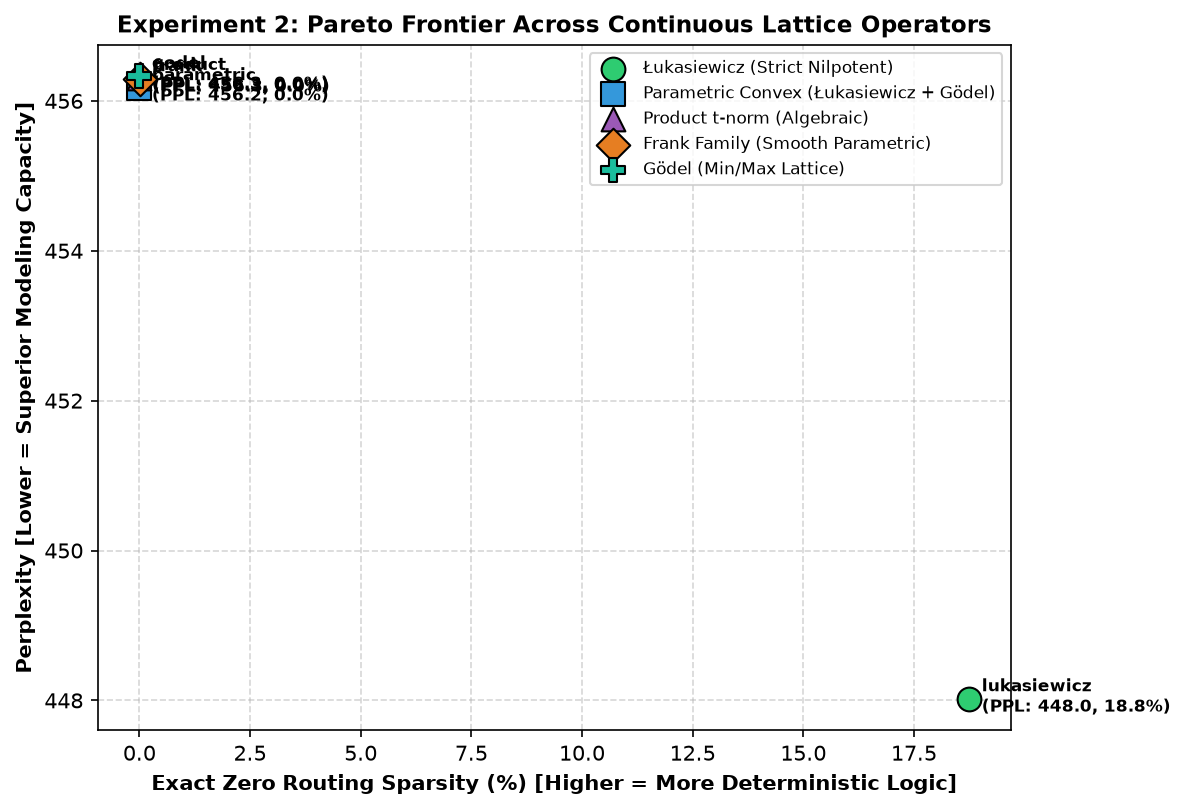
\includegraphics[height=1.85cm, keepaspectratio]{exp2_operator_pareto.png}
\caption{Exp 2: Operator Pareto Frontier.}
\label{fig:exp2_pareto}
\end{minipage}
\hfill
\begin{minipage}{0.48\textwidth}
\centering
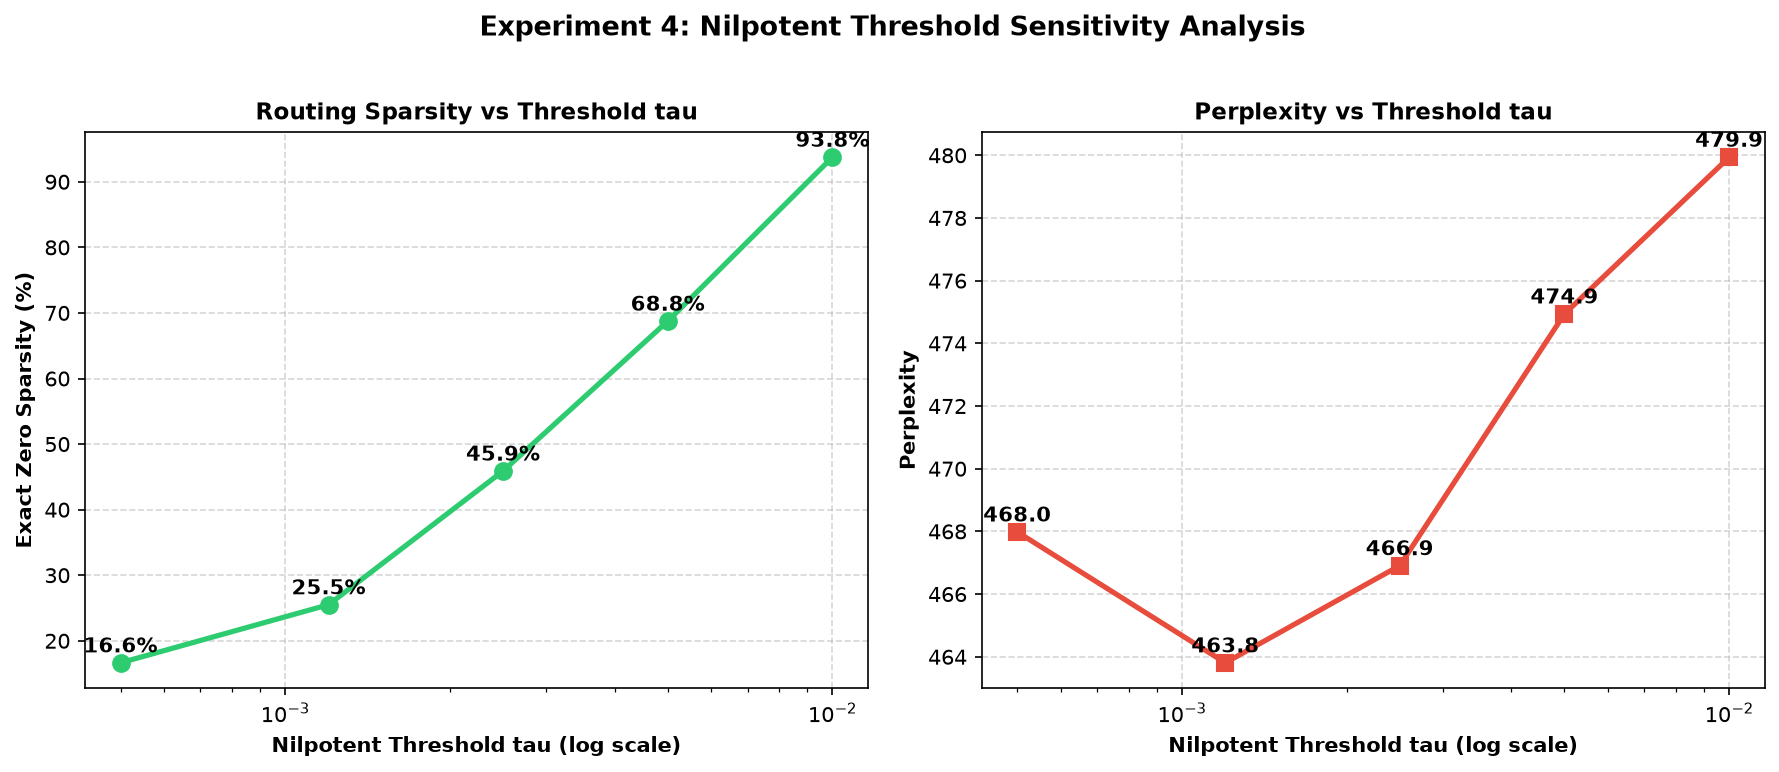
\includegraphics[height=1.85cm, keepaspectratio]{exp4_tau_sensitivity.png}
\caption{Exp 4: Threshold $\tau$ vs. Sparsity.}
\label{fig:exp4_tau}
\end{minipage}
\end{figure}

\subsection{Exp 5: Initial Hallucination Stress Test}
When distractor sentences were inserted into WikiText-2, the baseline allocated 70.10\% of its attention to distractors. Soft L-Topology pruned \textbf{25.00\% of distractor connections to exact 0.0000}, cutting distractor leakage to 45.17\% (a 24.93\% absolute noise reduction).
